\chapter{Discussion}
\label{chap:discussion}

\section{Applicability of the eye tracking framework on the target group}
\label{sec:discapplicability}

Regarding the research question 3.a (\textit{was it possible to conduct the experiment until the end?}), only P1 managed to reach the last trial, but she did not complete it fully. P2 and P3 lost interest at the third trial, not performing the last one. At the current state of the experimental design, it seems that it lasts a bit too long. Both the stimuli and also the interstimulus materials should be shorter. Shortening the stimuli presentation means showing less repetitions of the stimuli or shortening the durations of expected fixations, if the other parameters of frequency and velocity (particularly important for smooth pursuit) and size of the stimulus remain constant. Lowering the number of repetitions could make the stimuli provide less repeated measurements and therefore less assessments for internal consistency and less reliability of the measurements in general. However, it is probably better to have less repeated measurements than not having measurements at all, as happened for Trial 4, which was not performed by P2 and P3.

Regarding the research question 3.b (\textit{was the percentage of tracking ratio for each visual stimuli \textgreater 50\%?}), 6 out of a total of 12 trials have tracking records for more than half of the total time of the presentation of the stimuli. The tracking ratio percentage does not describe the quality of the data, but it provides a good index of how efficient the eye tracker in collecting data during the experiments. Considering the lack of control over every potential distractor in the environment (e.g. participants children free to move while sitting on the lap of their caregiver, people free to pass by the experiment location, researchers out of the sight of the participant but still present in the location, etc) and the fact that probably the stimuli lasted for a bit longer than the necessary (increasing the total amount of time which the tracking ratio percentage refers to), collecting data for half of the trials can be considered satisfactory for this first experimentation. P1 (15 months of age) and P2 (24 months of age) data records already show noticeable high percentages of tracking ratio, and indeed their records are pretty complete in some tasks. All the participants though show a decrease of tracking ratio the more the experiment proceeded, resulting also in P2 and P3 not performing the last task. P3 (9 months of age) records are overall much shorter than P1 and P2. This might be due to a series of factors (e.g. a shorter attention spans at her very young age, more difficulties to sit still for long periods of time) but, regardless the motivation, the procedure collected more data for the two children in the target age group than the younger one.
The research question 3.c (\textit{is the percentage of repetitions performed entirely over the total number of repetition displayed \textgreater 50\%?}) is closely related with 3.b, but it tells more about the quality of the recorded data rather than the quantity. As explained before, the number of repetitions is important to ensure reliable measurements. 4 out of 12 trials collected tracking records of at least half of the repetitions designed in the visual stimuli, indicating that very frequently the children lost interest in the stimuli or started to behave differently (e.g. moved to far away from the experiment computer or sat in different positions) during the stimuli presentation. Looking at the percentages of repetitions performed for each stimuli, it does not emerge a preference for a particular visual stimuli, which could have hypothetically scored systematically better, eliciting more repetitions than others. From the graphs does not seem to emerge a particular moment in which the children stopped following some repetitions. Indeed, the participant’s mothers tried to redirect the children’s attention towards the screen while they felt the babies were looking elsewhere. Their intervention helped in collecting further eye recordings and possibly further repetitions, but in absence of video recordings it prevents to pinpoint the exact moments in which the children lost interest at first. However, it was evident in during the experimentation that the partnership with the mothers was fundamental both in making the children feel more at ease and also to collect more eye movement data.

Regarding the research questions 3.b and 3.c, a possible further step for refining the framework is to shorten the stimuli and the interstimulus materials, and to reduce a bit the number of repetitions for each stimuli. This operation should increase the number of repetitions performed and therefore also the tracking ratio over all the experiment duration.
While the performance metrics (related to 3.a, 3.b and 3.c) highlight the need of further refinement of timing and conciseness of the stimuli and interstimulus materials, probably the most interesting results of this experimentation are related to the research question 3.d (\textit{Do the diagrams of the eye tracking data show qualitatively the gaze patterns which the methods were aimed to elicit?}). Regardless of the amount of eye tracking data or repetitions, in the charts of 9 out of 10 total performed trials (2 are missing) it is possible to detect the correct gaze patterns under investigation. Even in the records of P3, which overall show few segments of the trials, the gaze patterns recorded were actually quite similar to the expected ones. These results suggest that the design of the visual stimuli is appropriate for eliciting the eye parameters of interest, at least in children between 9 and 24 months of age with no vision problems or any clinical diagnosis. They were interesting enough to elicit at least some visual tracking, and with some external reinforcement coming from the caregiver, the children did actually perform the expected gaze patterns. Therefore, as a further step in the research it is probably the procedure which needs to be refined more than the visual stimuli.

Summarizing, answering the research question 3, the outlined procedure seems to be applicable to children in the target age group 12-24 months, and with some major improvements probably even on younger children too. The timing and the duration of the stimuli and interstimulus materials seems to be the crucial point to fix, but the stimuli seem to elicit the correct eye movements.

\section{Considerations about the data recordings, stimuli and process }
\label{sec:discconsiderations}

During the experiments some further interesting elements emerged, which need to be taken into consideration for further developments of the framework.

In the pilot test trials it is quite evident that the left eye of the subject followed the targets with greater stabilization, and perhaps more accuracy, suggesting its dominance over the right eye. Therefore it would be probably more useful to analyze only the left eye records in order to compute performance metrics and having clearer results. In the charts from the experimental group, the children’s eyes do not show this pattern as clear as PT, and therefore it would be necessary compute the records of both the eyes or determining each time what it seems to be the dominant eye record. Basing on the plotted charts, it is possible that at the young age of the experimental group the eye dominance mechanism is still not evident as much as in adults.

The “staircase” profile firstly shown by P1 (P1\_T1, Fig.~\ref{fig:P1_T1_pos}; P1\_T2, Fig.~\ref{fig:P1_T2_pos}) could be due to the fact that the velocity of the target smooth movement was too quick, therefore it required the P1’s saccadic system to intervene during the target tracking. P2 did not show this staircase profile (P2\_T1, Fig.~\ref{fig:P2_T1_pos}; P2\_T2, Fig.~\ref{fig:P2_T2_pos}), while P3 did (P3\_T1, Fig.~\ref{fig:P3_T1_pos}; P3\_T2, Fig.~\ref{fig:P3_T2_pos}). These data suggest that, perhaps, the autonomy of the smooth pursuit system develops after 15 months of age towards the 24 months. Before 15 months of age, the smooth pursuit system does still not perform in complete autonomy, and it still interacts with the saccadic system noticeably, or maybe it works more precisely and autonomously at slower target velocities than the ones tested. Indeed, \cite{falck-ytter2013eyetrackingASD} report that vertical and two-dimensional tracking matures over the first years of life.

Regardless the physiological explanation of the behavior, it is probably necessary to generate smooth pursuit sinusoidal and triangular visual stimuli with slower target velocities, at least for the younger age ranges in the target group. This should allow the children’s smooth pursuit systems to attune better to the target and to prevent the saccadic systems to intervene and to add noise to smooth pursuit data.
P1 and P3 data also show the staircase profile during the Step-Ramp visual stimuli (P1\_T3, Fig.~\ref{fig:P1_T3_pos}; P3\_T3, Fig.~\ref{fig:P3_T3_pos}), but only in some parts of the chart and with less intensity. This might be due to the fact that the motion in this stimuli happens only on the horizontal axis. Therefore it is probably less complex for the children to attune their eye movement to such stimuli, comparing to the sinusoidal or triangular target motions.

From the data collected for P1\_T4 (Fig.~\ref{fig:P1_T4_pos}), it should be technically possible to compute the standard deviation of the saccade gain with an appropriate calculation module. Regardless the data noise shown during the fixations, which is not of interest for the framework, the visually guided saccades appear to have clean and well isolated velocity profiles in the record. In the future, isolating systematically these eye velocity profiles and comparing them with the velocity should be doable, and it would be definitely less challenging than computing smooth pursuit metrics.

Some practical issues emerged during this first series of experiments. If the location in which the experiment takes place is too bright, calibrating the eye tracker reveals to be challenging. In order to avoid to change locations multiple times in an home environment, it is beneficial to ask upfront directly to the caregivers or the owners of the facility about which location could be the most suitable one, and if they are available.

Instructing the caregivers about what they can do to support the experiments (e.g. redirect the children’s attention toward the screen if they start to focus elsewhere) and what is their level of freedom (e.g. feel free to talk, move and play with the child during the interstimulus material presentation) is of utmost importance. They should feel to be research partners and stakeholders in the process. Their collaboration directly impacts on the amount of recorded data, and therefore the overall efficiency and effectiveness of the procedure.

Even if during the experiments the researchers tried to place themselves out of the participants’ sight and to control remotely the computer, their presence was still a big distraction for the participants. Being strangers in an home environment surely catches everyone's attention. Even if the procedure is carried out at a clinical facility, it should be expected that the children would be at least a bit curious toward the people around them. In the future, it will be important to set up a series of remote controlling devices, connected via wireless (either Wi-Fi or even better local Bluetooth) to the experiment computer, which allows to see a streaming of the children’s behavior and to control the experiment software from an another remote device, which could be even a tablet or a smartphone for example. This would allow the researchers to sit at a fair distance from the experiment location, preventing to add unnecessary distractions, and at the same time control when the child seems not interested anymore in the stimuli, and therefore move forward with the experiment. If the researchers can setup a dedicated location for the experiments, having more control over the layout and furnishing, an alternative option could be the one proposed by \cite{sasson2012children}, that is placing a partition between the eye-tracking station and the computer operated by the experimenters, with a camera showing a view of the participant. This kind of arrangement is very near to the one illustrated by \cite{anderson2006visualscanning}(Fig.~\ref{fig:partitionsetup}).

\begin{figure}[h]
  \centering
  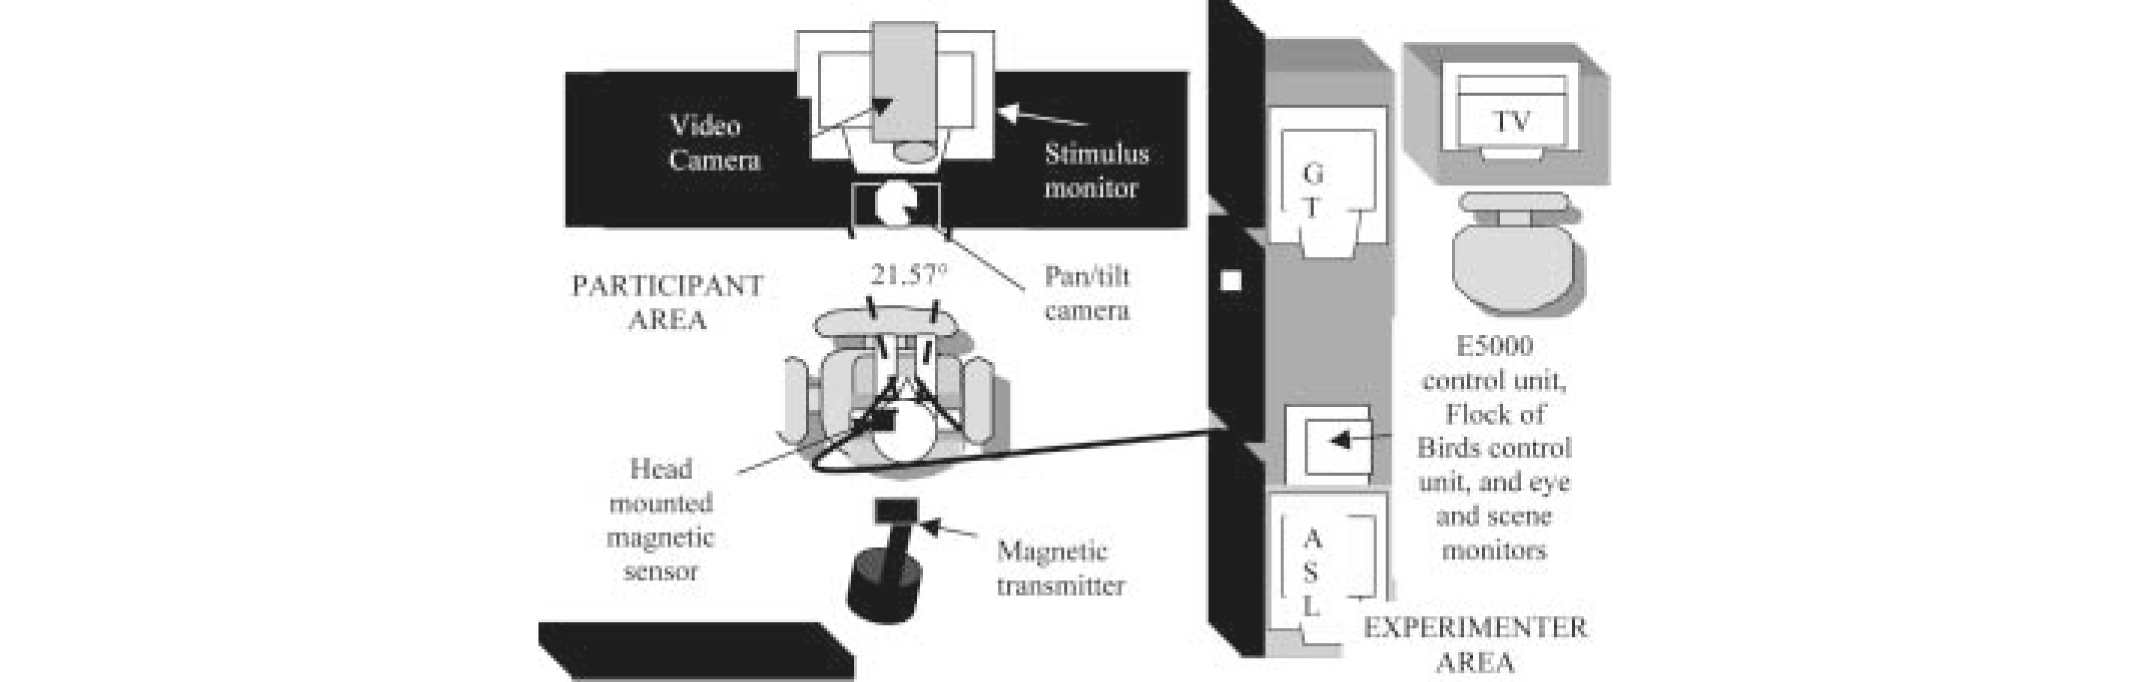
\includegraphics[width=.9\textwidth]{figures/andersonpartition-13.jpg}
  \caption[Example of partition setup]{Experimental setup with a partition between participants and experimenters. Scheme taken from \cite{anderson2006visualscanning}}
  \label{fig:partitionsetup}
\end{figure}